%%%%%%%%%%%%%%%%%%%%%%%%%%%%%%%%%%%%%%%%%%%%%%%%%%%%%%%%%%%%%%%%%%%%%%%%%%%%%%%%%%%%%%%%%%%%
%%
%% Chapter 3 : Related works
%%
%%      * Should give an overview of what the big dogs are saying in the field
%%
%%  BASIC STRUCTURE :
%%
%%      a. Current benchmarks for robot locomotion
%%          * DeepMind's ControlSuite
%%          * OpenAI's mujoco-py
%%          * Berkeley's garage and rllab
%%          * Stanford's robosuite
%%          * NVIDIA Isaac + FleX
%%          * UBC's terrainRlSim
%%          * Unity's ml-agents (talk about the marathon envs)
%%
%%      b. DRL algorithms for robot locomotion
%%          * Benchmarking drl for continuous ccontrol (2016?)
%%          * Trust region policy optimization
%%          * Proximal policy optimization
%%          * DeepTerrainRL
%%          * DeepLoco
%%          * DeepMimic
%%          * Emergence of locomotion in rich and complex environments
%%
%%%%%%%%%%%%%%%%%%%%%%%%%%%%%%%%%%%%%%%%%%%%%%%%%%%%%%%%%%%%%%%%%%%%%%%%%%%%%%%%%%%%%%%%%%%%


\chapter{Related Works}
\label{ch:relatedWorks}

%%%%%%%%%%%%%%%%%%%%%%%%%%%%%%%
%   Figures for chapter 3 - 
%%%%%%%%%%%%%%%%%%%%%%%%%%%%%%%

%% \newcommand{\figFrameworkFlow}{
%%     \begin{figure}
%%         \centering
%%         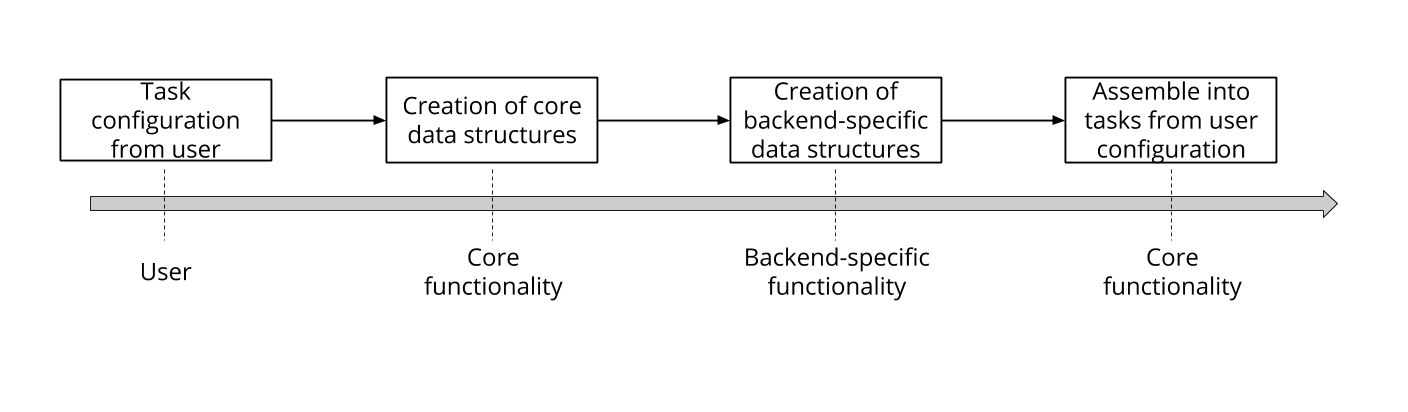
\includegraphics[width=0.9\textwidth]{./chapters/chapter_4/imgs/img_ch4_framework_flow.png}
%%         \caption{Flow of data in the proposed framework}
%%         \label{fig:ch4_proposed_framework_flow}
%%     \end{figure}
%% }

%% \newcommand{\figFrameworkCoreSensor}{
%%     \begin{figure}[!ht]
%%         \centering
%%         \begin{subfigure}[b]{0.3\textwidth}
%%             \centering
%%             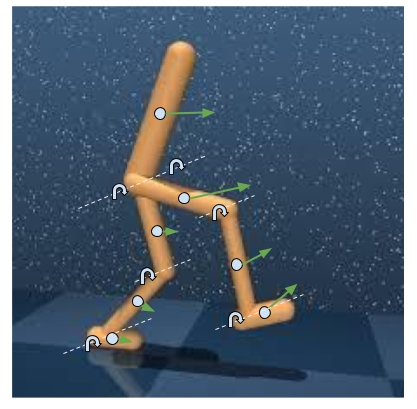
\includegraphics[width=0.9\textwidth]{./chapters/chapter_4/imgs/img_ch4_sensors_core_1.png}
%%             \caption{}
%%             \label{fig:ch4_core_sensor_1}
%%         \end{subfigure}
%%         \begin{subfigure}[b]{0.3\textwidth}
%%             \centering
%%             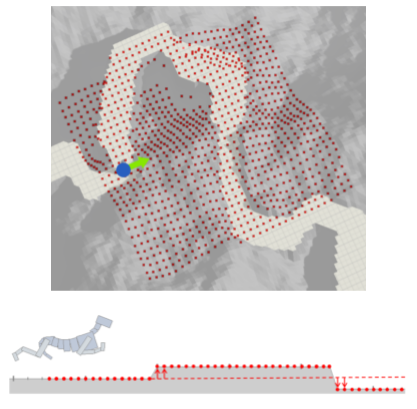
\includegraphics[width=0.9\textwidth]{./chapters/chapter_4/imgs/img_ch4_sensors_core_2.png}
%%             \caption{}
%%             \label{fig:ch4_core_sensor_2}
%%         \end{subfigure}
%%         \begin{subfigure}[b]{0.3\textwidth}
%%             \centering
%%             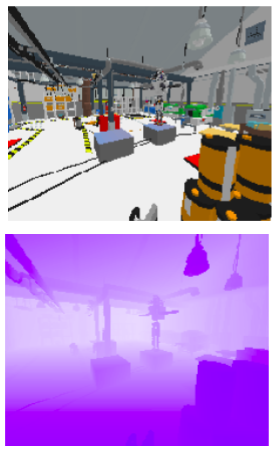
\includegraphics[width=0.9\textwidth]{./chapters/chapter_4/imgs/img_ch4_sensors_core_3.png}
%%             \caption{}
%%             \label{fig:ch4_core_sensor_3}
%%         \end{subfigure}
%%         \caption{Core sensors functionality. a) Intrinsic readings from joints and bodies (adapted from [@CITE]).
%%                                              b) Extrinsic readings from heightmaps of the terrain (adapted from [@CITE,@CITE]).
%%                                              c) Extrinsic readings from rgb and depth images of the agent view (adapted from [@CITE]).}
%%         \label{fig:ch4_core_sensor_functionality}
%%     \end{figure}
%% }

\newcommand{\figPolicyChanges}{
    \begin{figure}[!ht]
        \centering
        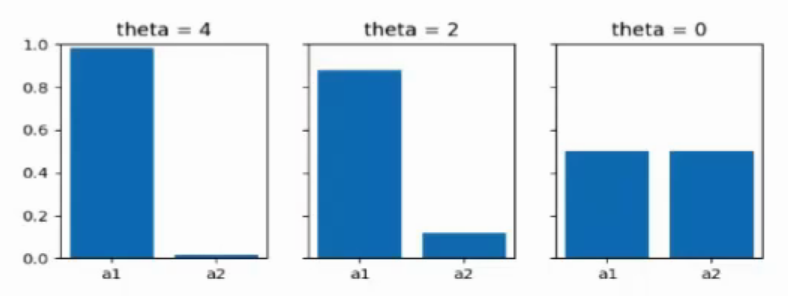
\includegraphics[width=0.8\textwidth]{./chapters/chapter_3/imgs/img_ch3_euclidean_constraint.png}
        \caption{A simple example that shows that same changes in parameter space yield 
                 very different changes in policy space. Adapted from \href{https://youtu.be/yqYKeWtUSO8?t=1050}{this} lecture.}
        \label{fig:ch3_policy_changes}
    \end{figure}
}

\newcommand{\figBenchmarkControlSuite}{
	\begin{figure}
		\centering
		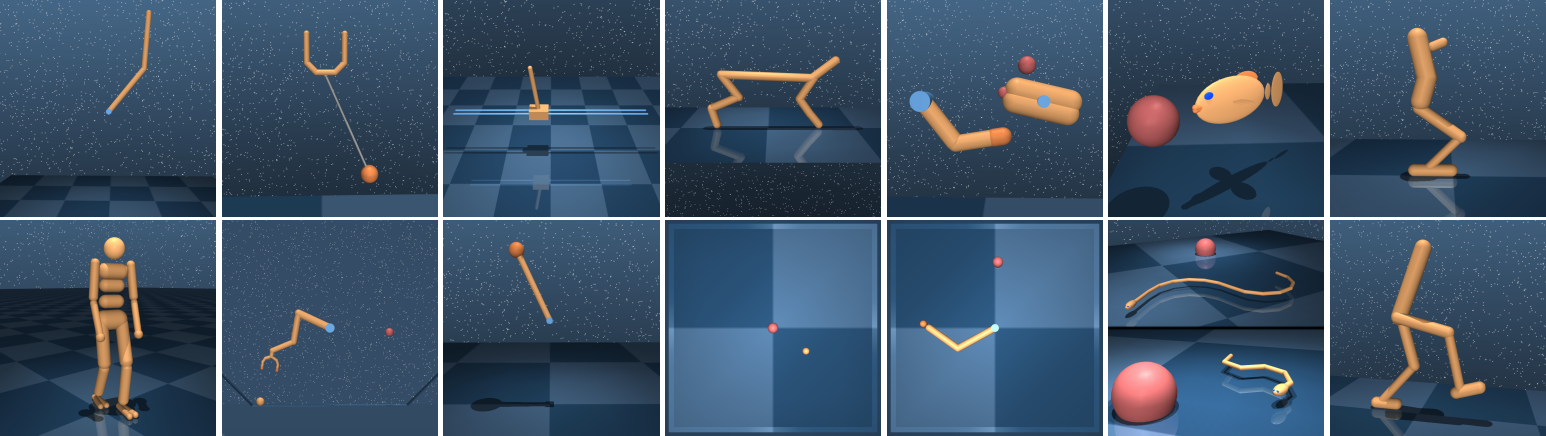
\includegraphics[width=0.9\textwidth]{./chapters/chapter_3/imgs/img_ch3_controlsuite.png}
		\caption{Models available in the Controlsuite benchmark. 
				 Extracted from \citet{Controlsuite}}
	    \label{fig:ch3_controlsuite}
	\end{figure}
}

\newcommand{\figBenchmarkOpenAIGymMujoco}{
    \begin{figure}[!ht]
        \centering
        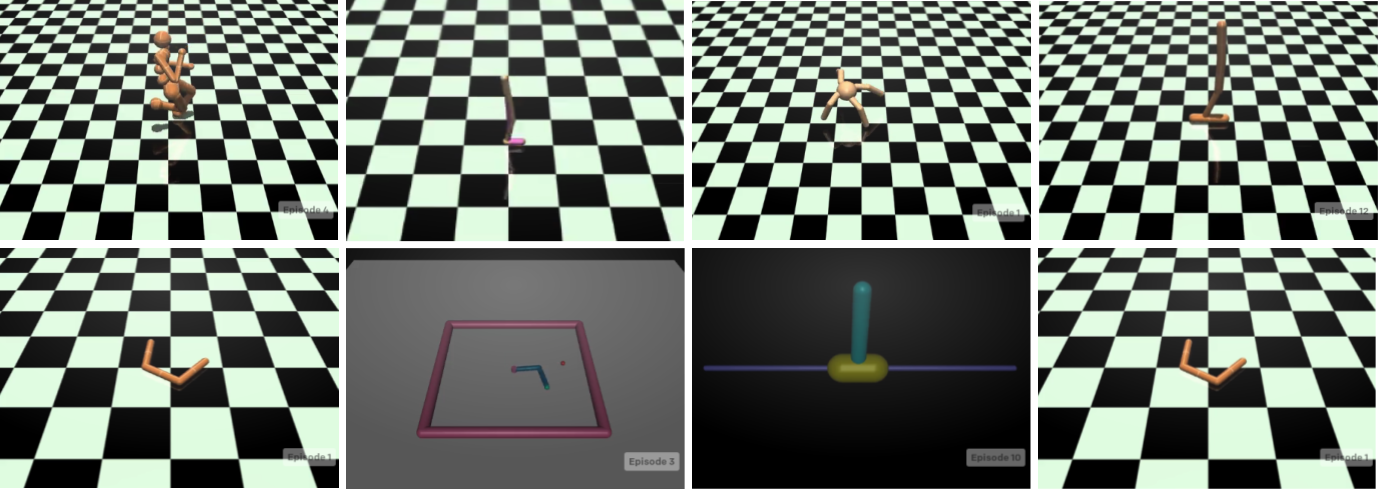
\includegraphics[width=0.9\textwidth]{./chapters/chapter_3/imgs/img_ch3_openaigym_mujoco.png}
        \caption{Models available in the OpenAI-gym benchmark with mujoco as backend. 
                 Extracted from \citet{Gym}}
        \label{fig:ch3_openaigym_mujoco}
    \end{figure}
}

\newcommand{\figBenchmarkOpenAIGymRoboschool}{
    \begin{figure}[!ht]
        \centering
        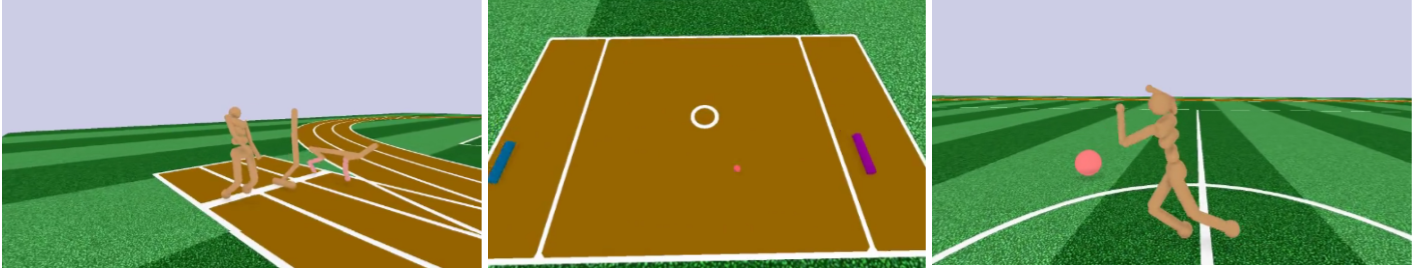
\includegraphics[width=1.0\textwidth]{./chapters/chapter_3/imgs/img_ch3_openaigym_roboschool.png}
        \caption{Models available in the OpenAI-gym benchmark with Bullet as backend. 
                 Extracted from \citet{Roboschool}}
        \label{fig:ch3_openaigym_roboschool}
    \end{figure}
}

\newcommand{\figBenchmarkRllabClassic}{
    \begin{figure}[!ht]
        \centering
        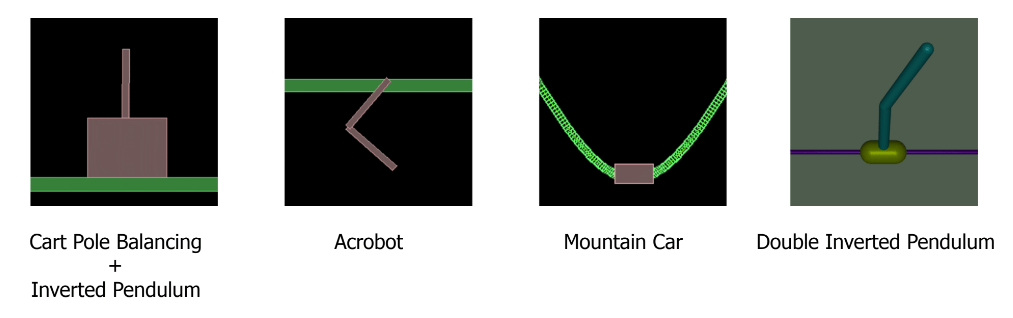
\includegraphics[width=0.9\textwidth]{./chapters/chapter_3/imgs/img_ch3_rllab_classic.png}
        \caption{Models available in the Rllab classic benchmark. Extracted from \cite{Rllab}}
        \label{fig:ch3_rllab_classic}
    \end{figure}
}

\newcommand{\figBenchmarkRllabLocomotion}{
    \begin{figure}[!ht]
        \centering
        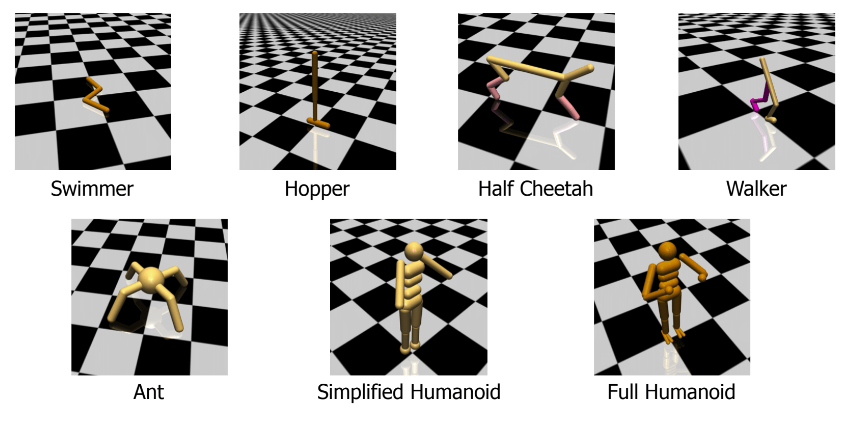
\includegraphics[width=0.9\textwidth]{./chapters/chapter_3/imgs/img_ch3_rllab_locomotion.png}
        \caption{Models available in the Rllab locomotion benchmark. Extracted from \citet{Rllab}}
        \label{fig:ch3_rllab_locomotion}
    \end{figure}
}

\newcommand{\figBenchmarkRllabHierarchical}{
    \begin{figure}[!ht]
        \centering
        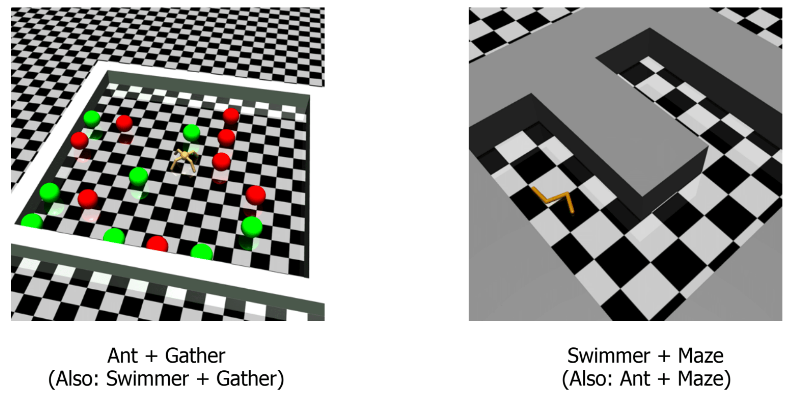
\includegraphics[width=0.9\textwidth]{./chapters/chapter_3/imgs/img_ch3_rllab_hierarchical.png}
        \caption{Models available in the Rllab hierarchical benchmark. Extracted from \citet{Rllab}}
        \label{fig:ch3_rllab_hierarchical}
    \end{figure}
}

\newcommand{\figBenchmarksRobosuite}{
    \begin{figure}[!ht]
        \centering
        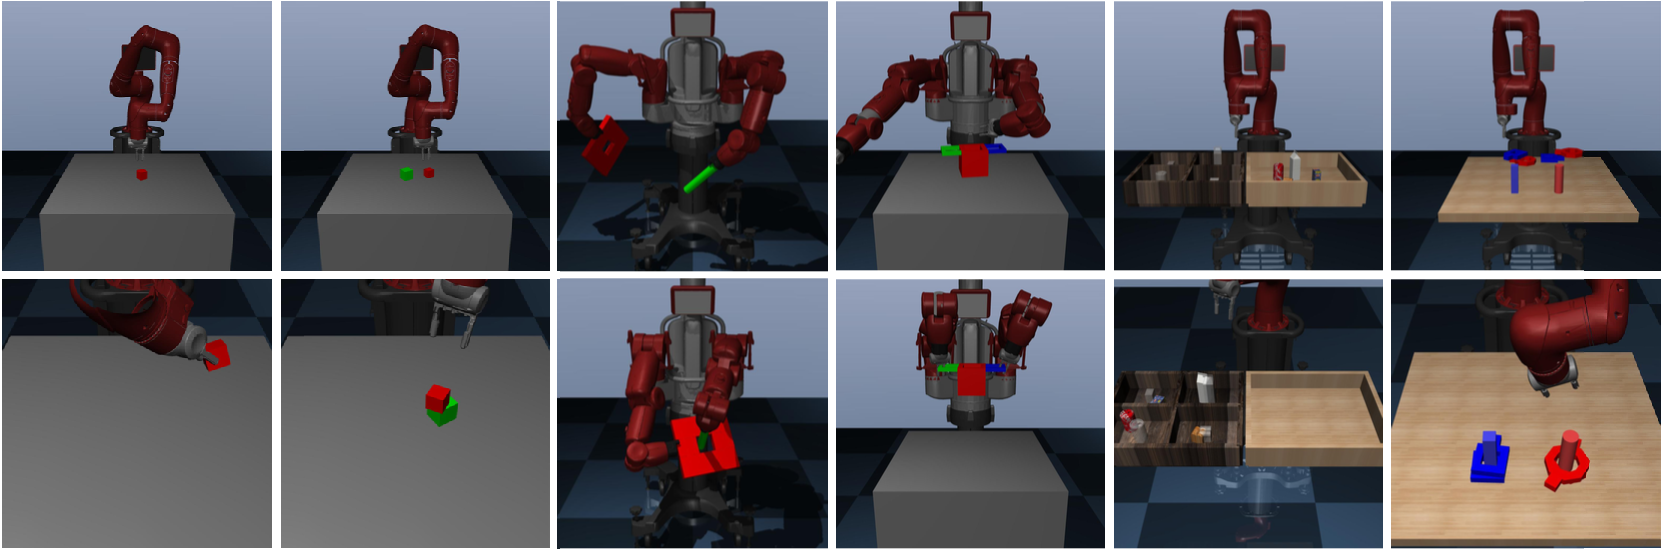
\includegraphics[width=1.0\textwidth]{./chapters/chapter_3/imgs/img_ch3_robosuite.png}
        \caption{Tasks available in Robosuite, as part of the Surreal framework \citep{Surreal}}
        \label{fig:ch3_robosuite}
    \end{figure}
}

\newcommand{\figBenchmarksGpuSim}{
    \begin{figure}[!ht]
        \centering
        \begin{subfigure}[b]{0.3\textwidth}
            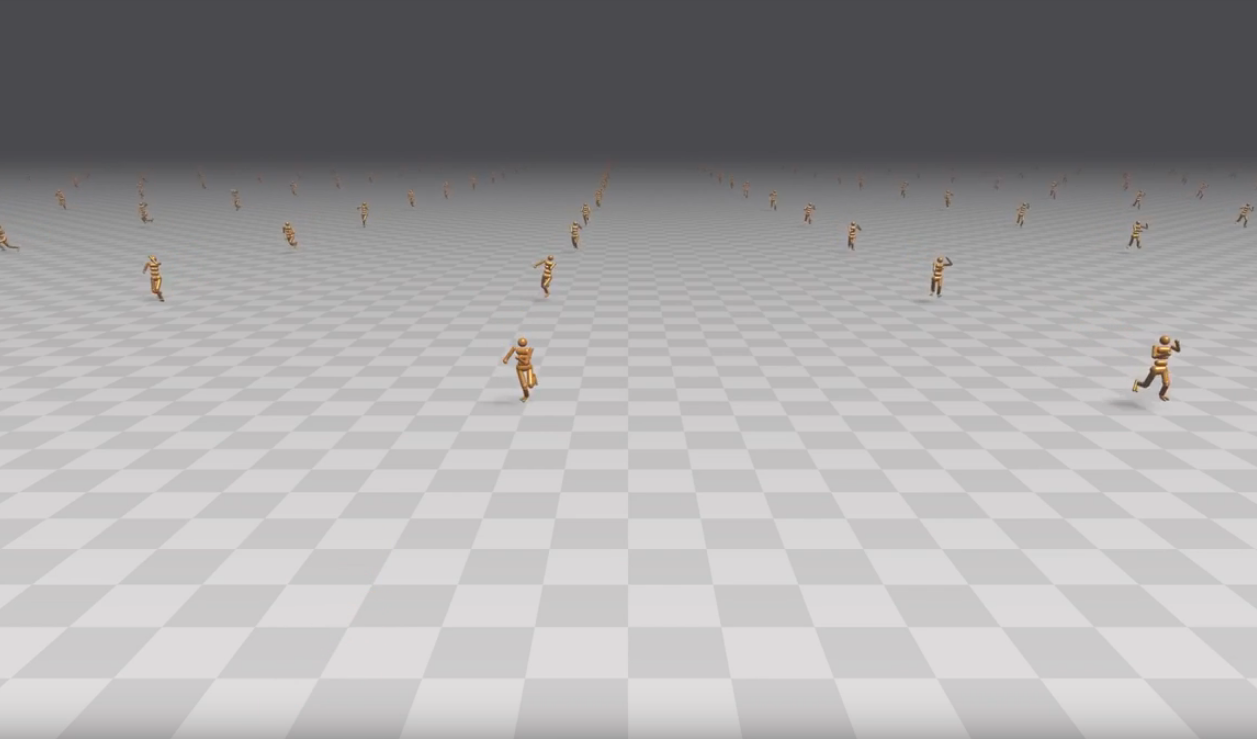
\includegraphics[width=1.0\textwidth]{./chapters/chapter_3/imgs/img_ch3_gpu_sim_1.png}
        \end{subfigure}
        \begin{subfigure}[b]{0.3\textwidth}
            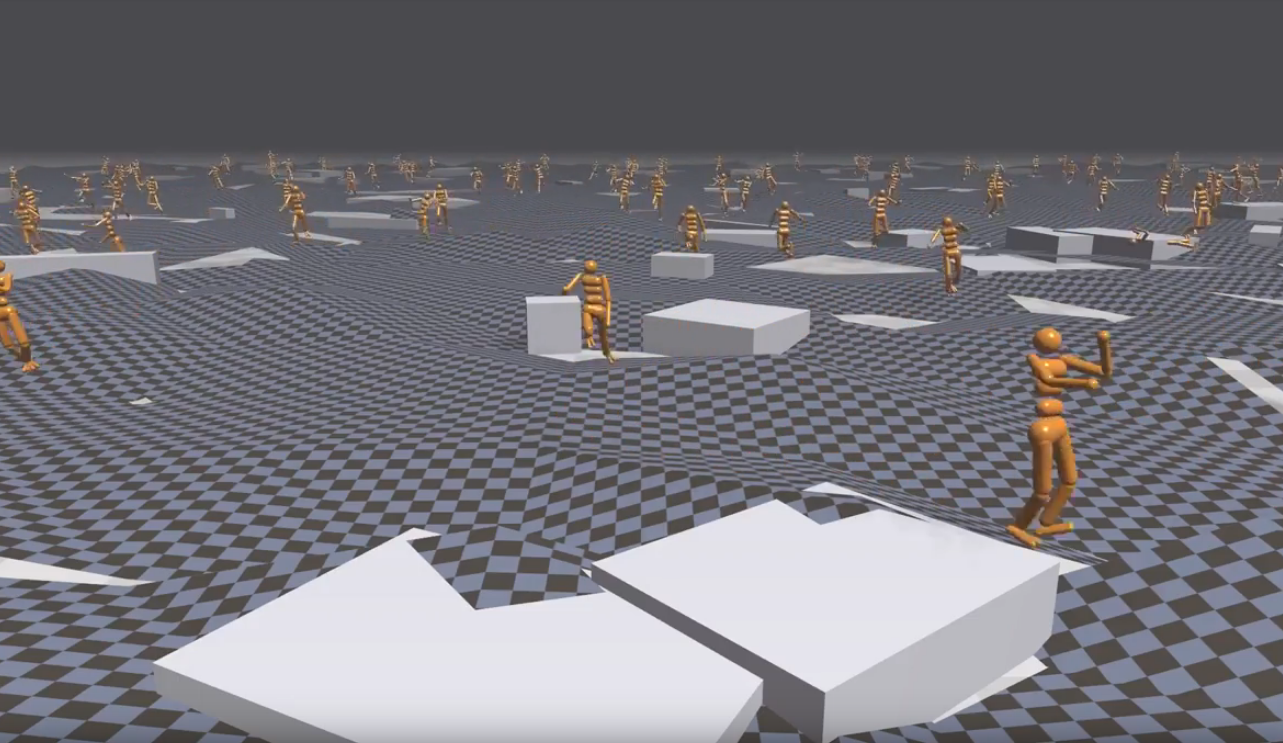
\includegraphics[width=1.0\textwidth]{./chapters/chapter_3/imgs/img_ch3_gpu_sim_2.png}
        \end{subfigure}
        \begin{subfigure}[b]{0.3\textwidth}
            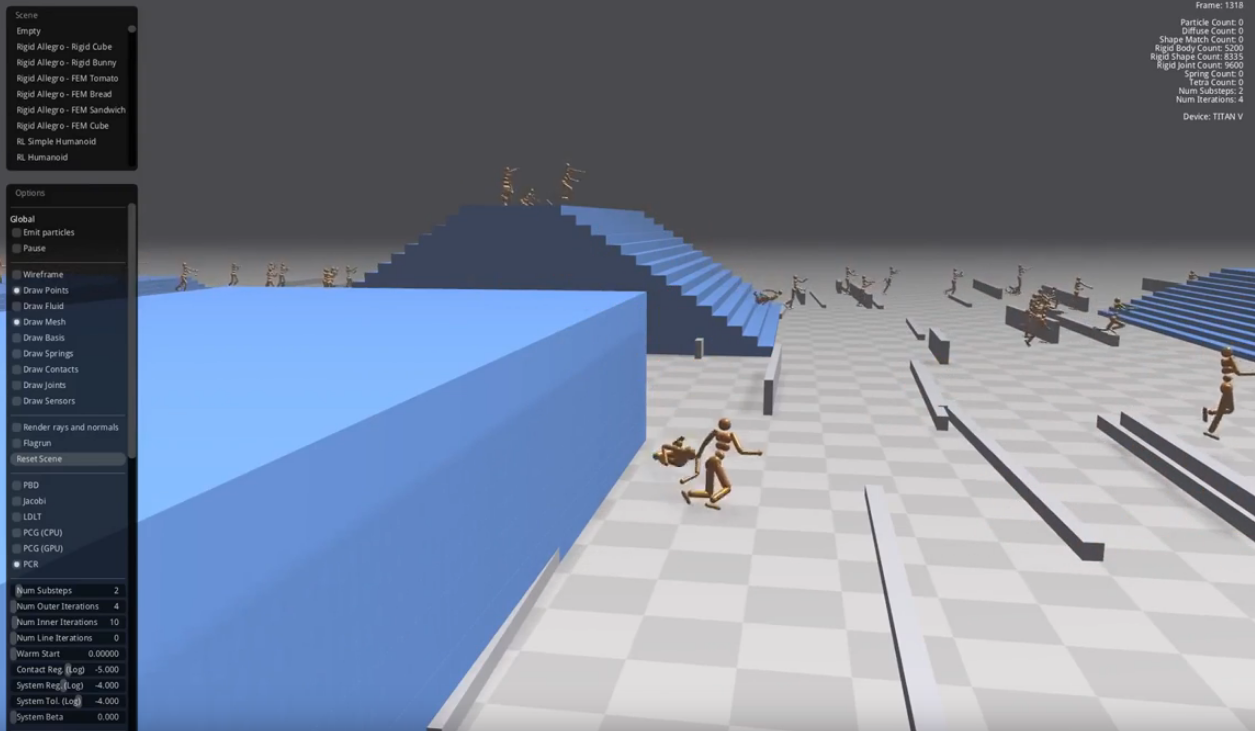
\includegraphics[width=1.0\textwidth]{./chapters/chapter_3/imgs/img_ch3_gpu_sim_3.png}
        \end{subfigure}
        \caption{Tasks provided in the Gpu-Accelerated simulator by \citep{GpuSim}}
        \label{fig:ch3_gpusim}
    \end{figure}
}

\newcommand{\figBenchmarksTerrainRLSim}{
    \begin{figure}[!ht]
        \centering
        \begin{subfigure}[b]{0.3\textwidth}
            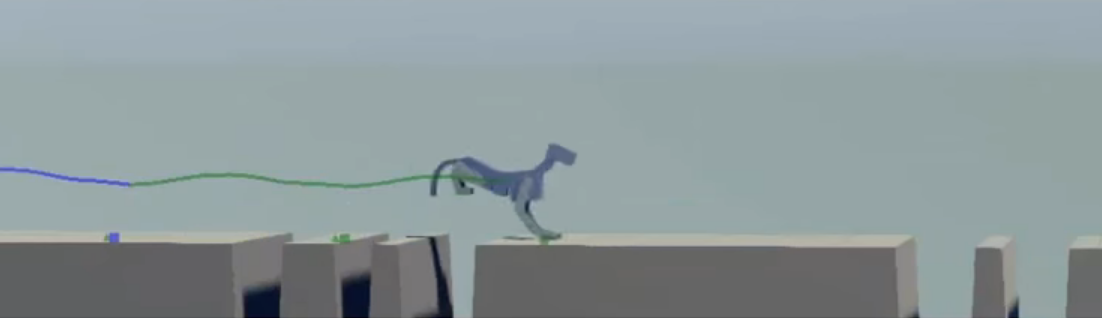
\includegraphics[width=1.0\textwidth]{./chapters/chapter_3/imgs/img_ch3_terrainrlsim_1.png}
            \caption{}
        \end{subfigure}
        \begin{subfigure}[b]{0.3\textwidth}
            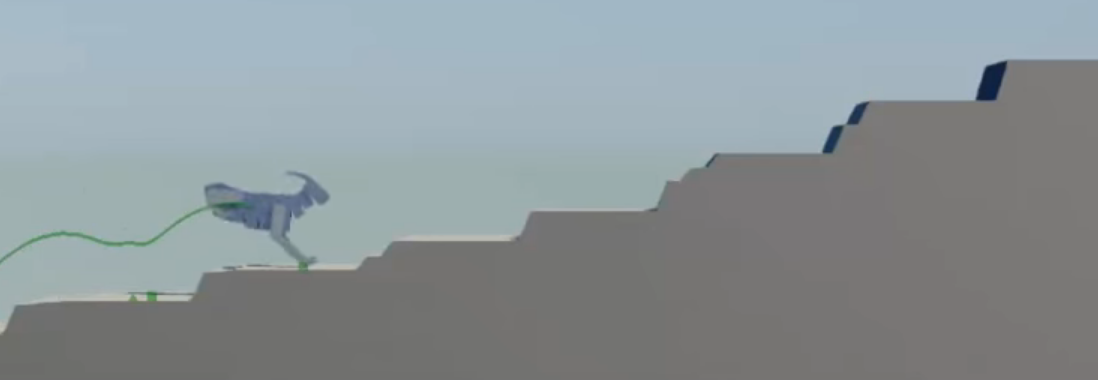
\includegraphics[width=1.0\textwidth]{./chapters/chapter_3/imgs/img_ch3_terrainrlsim_2.png}
            \caption{}
        \end{subfigure}
        \begin{subfigure}[b]{0.3\textwidth}
            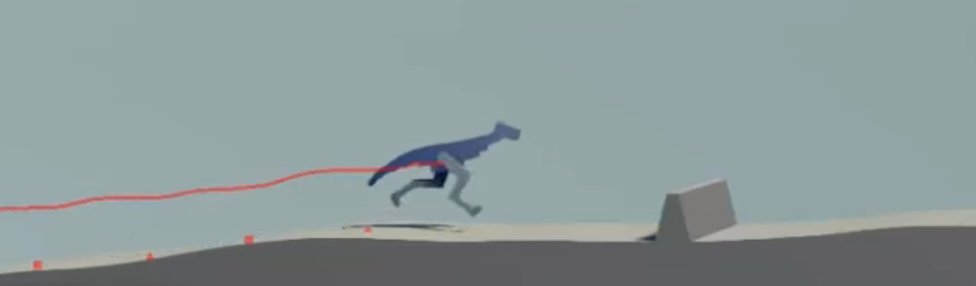
\includegraphics[width=1.0\textwidth]{./chapters/chapter_3/imgs/img_ch3_terrainrlsim_3.png}
            \caption{}
        \end{subfigure}

        \centering
        \begin{subfigure}[b]{0.3\textwidth}
            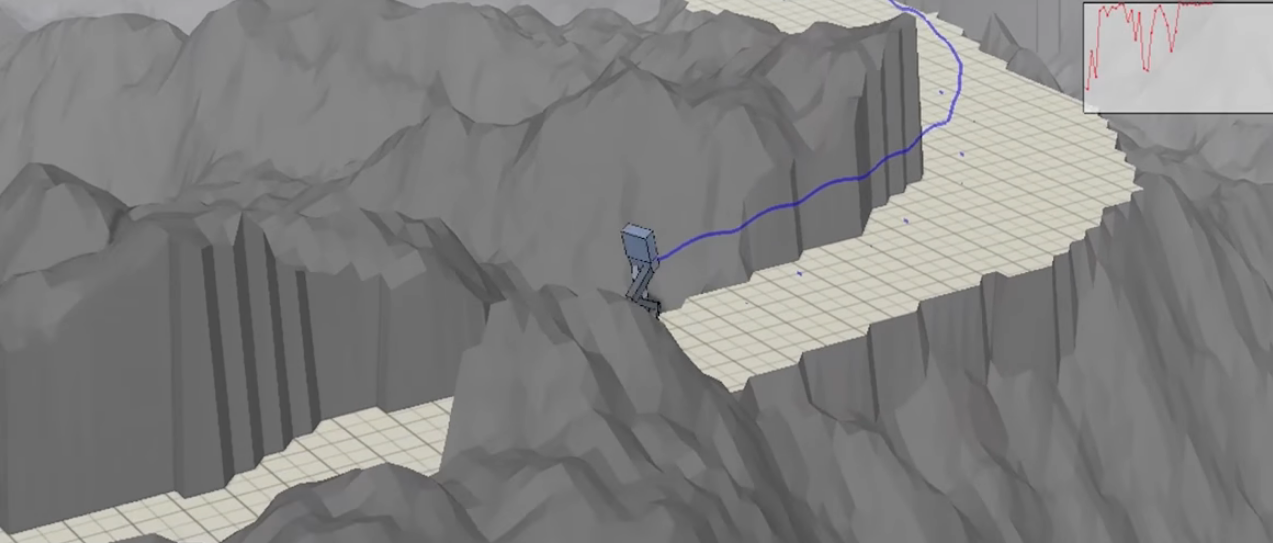
\includegraphics[width=1.0\textwidth]{./chapters/chapter_3/imgs/img_ch3_terrainrlsim_4.png}
            \caption{}
        \end{subfigure}
        \begin{subfigure}[b]{0.3\textwidth}
            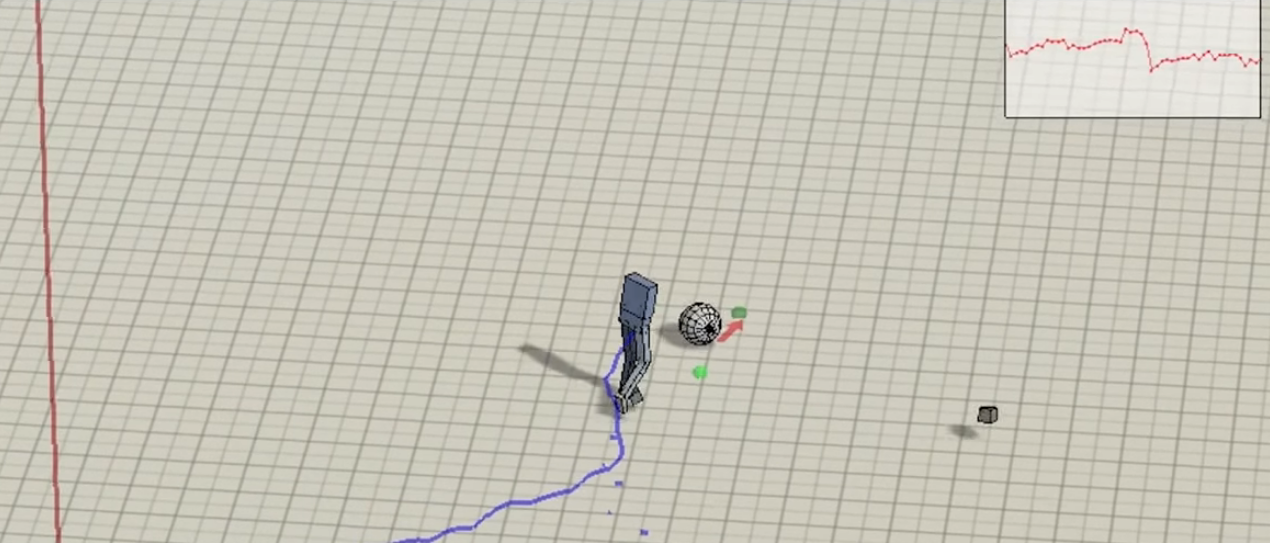
\includegraphics[width=1.0\textwidth]{./chapters/chapter_3/imgs/img_ch3_terrainrlsim_5.png}
            \caption{}
        \end{subfigure}
        \begin{subfigure}[b]{0.3\textwidth}
            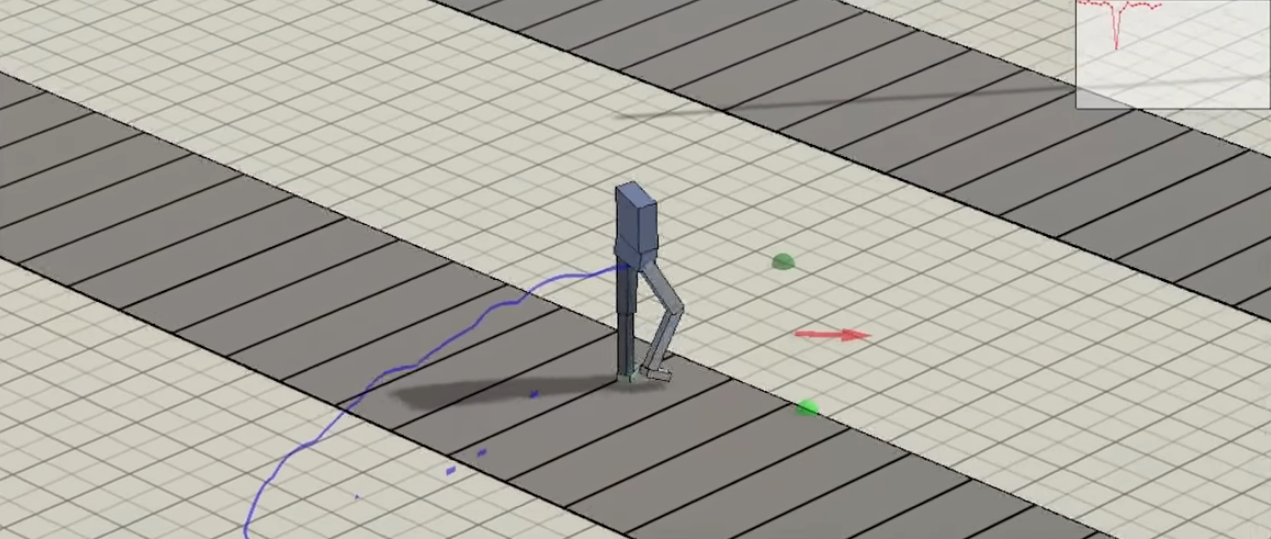
\includegraphics[width=1.0\textwidth]{./chapters/chapter_3/imgs/img_ch3_terrainrlsim_6.png}
            \caption{}
        \end{subfigure}

        \centering
        \begin{subfigure}[b]{0.3\textwidth}
            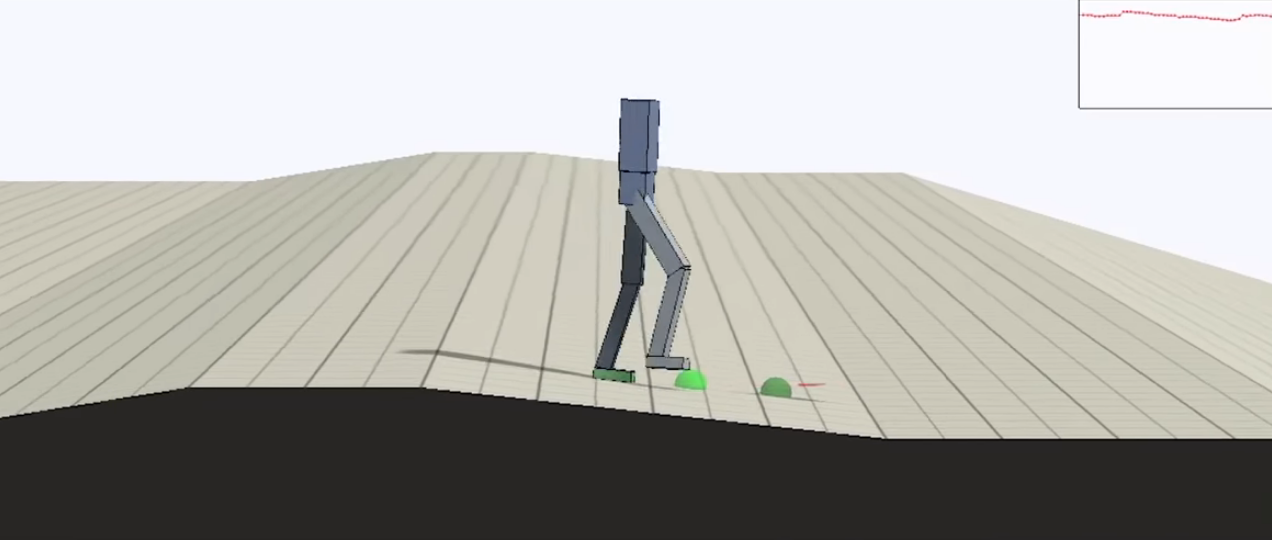
\includegraphics[width=1.0\textwidth]{./chapters/chapter_3/imgs/img_ch3_terrainrlsim_7.png}
            \caption{}
        \end{subfigure}
        \begin{subfigure}[b]{0.3\textwidth}
            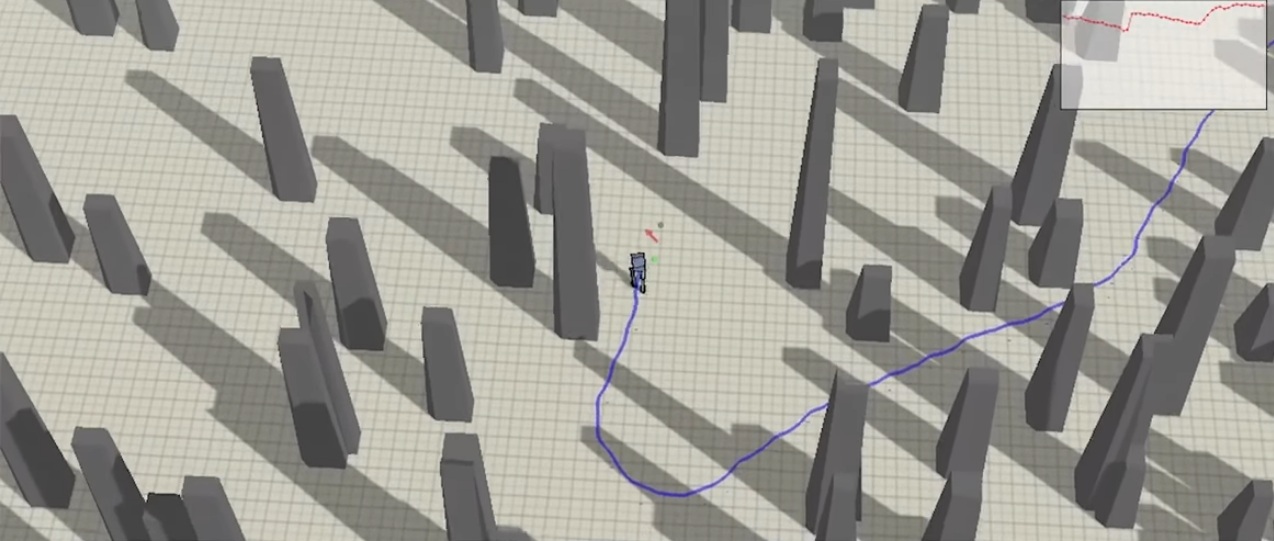
\includegraphics[width=1.0\textwidth]{./chapters/chapter_3/imgs/img_ch3_terrainrlsim_8.png}
            \caption{}
        \end{subfigure}
        \begin{subfigure}[b]{0.3\textwidth}
            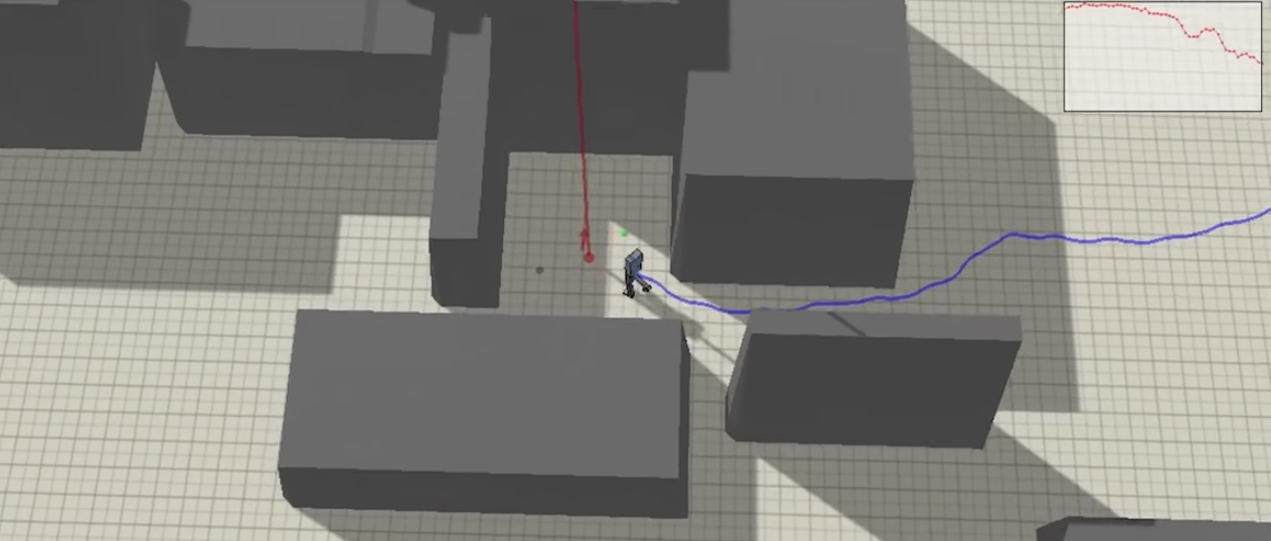
\includegraphics[width=1.0\textwidth]{./chapters/chapter_3/imgs/img_ch3_terrainrlsim_9.png}
            \caption{}
        \end{subfigure}

        \centering
        \begin{subfigure}[b]{0.3\textwidth}
            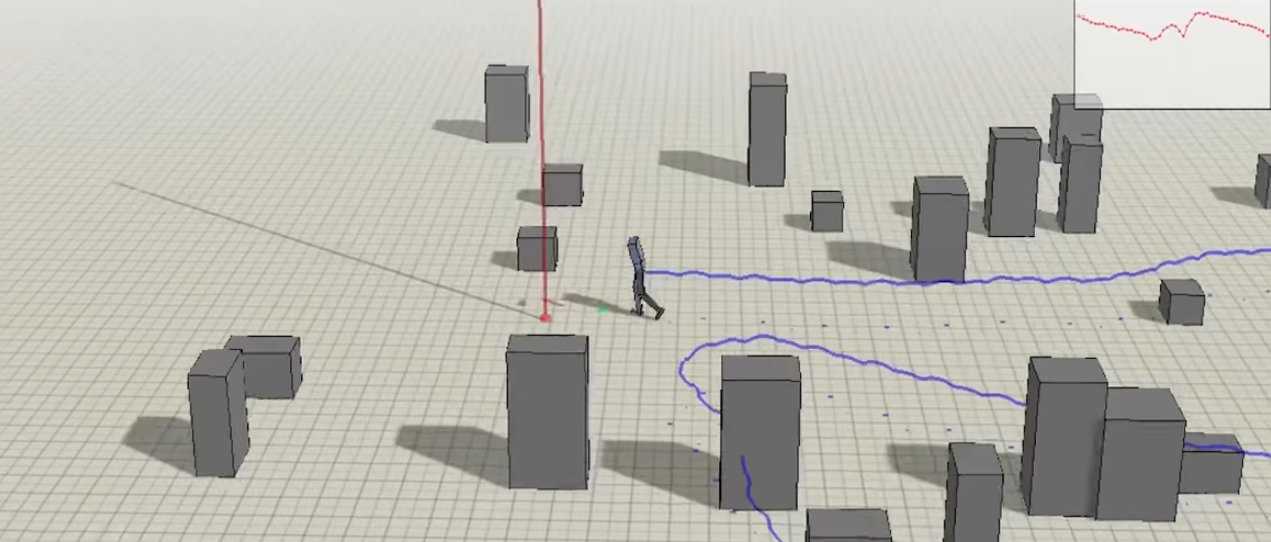
\includegraphics[width=1.0\textwidth]{./chapters/chapter_3/imgs/img_ch3_terrainrlsim_10.png}
            \caption{}
        \end{subfigure}

        \caption{Some of the tasks provided by the TerrainRLSim benchmark.}
        \label{fig:ch3_terrainrlsim}
    \end{figure}
}

\newcommand{\figBenchmarksUnityMLAgents}{
    \begin{figure}[!ht]
        \centering
        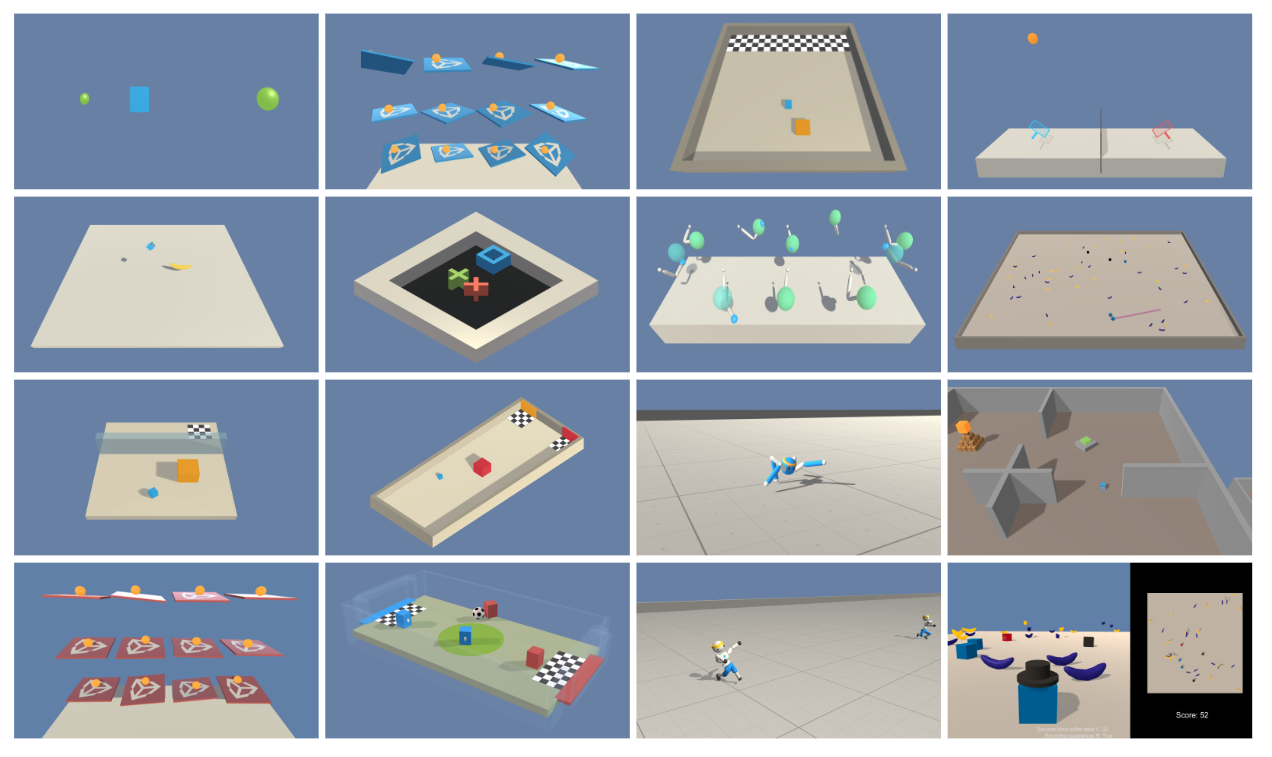
\includegraphics[width=1.0\textwidth]{./chapters/chapter_3/imgs/img_ch3_unity_ml_agents.png}
        \caption{Tasks available in the Unity ML-Agents framework.}
        \label{fig:ch3_unity_ml_agents}
    \end{figure}
}

\newcommand{\figBenchmarksMarathonEnvs}{
    \begin{figure}[!ht]
        \centering
        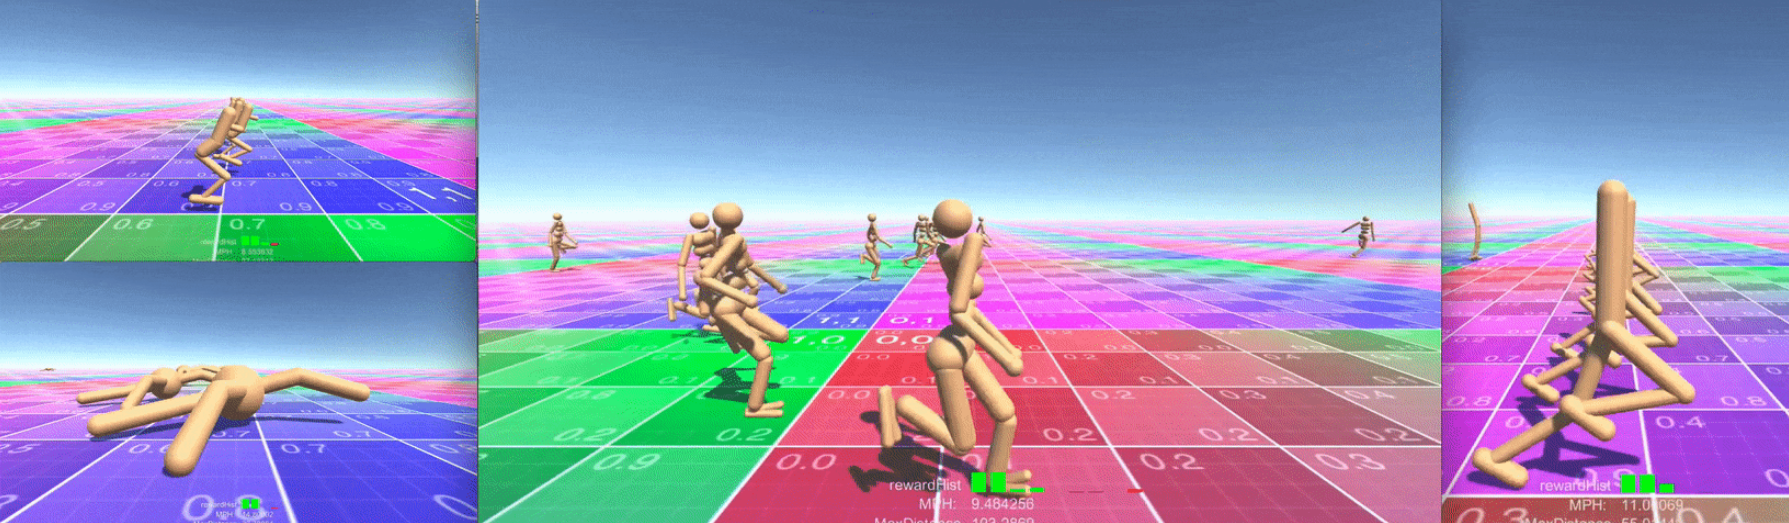
\includegraphics[width=1.0\textwidth]{./chapters/chapter_3/imgs/img_ch3_marathon_envs.png}
        \caption{Tasks available in the Marathon benchmark, provided along with the Unity ML-Agents framework.}
        \label{fig:ch3_marathon_envs}
    \end{figure}
}

\todo{Me preocupa un poco que la revision sea solo de herramientas, osea está muy orientado a eso, puede ser un punto en contra para un evaluador}
In this chapter we will give an overview of the currently available benchmarks
used for robot locomotion research. We give some high level details of the benchmarks,
which should help understand the proposal in Chapter 4.

%% In this chapter we will give an overview of the state of the art in robot locomotion using 
%% Deep Reinforcement Learning. We discuss some currently avaiable benchmarks for these tasks,
%% giving details that will help compare these current benchmarks with the proposed framework, which
%% will be discussed in more detail in chapter 4. We also discuss current state of the art algorithms
%% used to solve these tasks, which will be used as baselines for the experiments we will propose as part
%% of the evaluation procedure.

\section{Robot locomotion benchmarks}

\subsection{Deepmind ControlSuite}

This set of benchmarks was first introduced in \cite{Controlsuite}, and consists 
of various locomotion tasks (shown in Figure @FIG-3.1), with various types of agents 
to select from. The models available consist of xml files in the mujoco format (mjcf) 
that are used as the blueprints to instantiate an agent. The tasks consist of the specific
setups that the agents must solve, like walking, standing, running, etc.

\figBenchmarkControlSuite

As described in their \href{https://arxiv.org/pdf/1801.00690.pdf}{technical report},
some of the key features of this benchmark include:

\begin{itemize}
    \item \textbf{Full state observations}: the observations provided to the agent
          are sufficient to recover the full state of the environment. These observations
          include positions and velocities (of bodies and joints), touch sensor readings,
          and some other task specific measurements. Using this information, the full state
          of the environment can be recovered due to the simple nature of the environment 
          (most locomotion tasks in the benchmark are flat terrain tasks, and no information
          is hidden from the agents).

    \item \textbf{Normalized actions}: the actions exposed to the user have been normalized 
          in the range $\left[-1,1\right]$. These are mapped to actuators that represent
          torques applied to joints (torque actuation model).

    \item \textbf{Normalized rewards}: the rewards are set to the range $\left[ 0, 1 \right]$, 
          and can be smooth (whole range) or sparse (just the values $\left\{0,1\right\}$).

    \item \textbf{MuJoCo backend}: MuJoCo is the underlying physics backend, and it is
          integrated into the suite by using Python bindings generated using 
          \href{https://github.com/deepmind/dm_control/blob/master/dm_control/autowrap/autowrap.py}{ctypes}.
\end{itemize}

\subsection{OpenAI Gym}

This set of benchmarks consists of two separate options depending on the physics 
backend (MuJoCo and Bullet). These two options are Python Wrappers for the supported 
physics backends and are used as low level functionality for the high level API provided by Gym \citep{Gym}.
The options used as wrappers for the two physics backends available are the following:

\begin{itemize}
    \item \textbf{Mujoco-py} : A Python wrapper for MuJoCo, very similar to ControlSuite. 
          The available tasks are similar to the ones in ControlSuite, which are shown 
          in Figure @FIG-3.2.

        \figBenchmarkOpenAIGymMujoco

    \item \textbf{RoboSchool}: An implementation that uses PyBullet, which exposes 
          the Bullet physics engine through a Python API. The environments exposed 
          are a bit different to the previous suite, and are shown in Figure @FIG-3.3. 

        \figBenchmarkOpenAIGymRoboschool

\end{itemize}

The RL API exposed by Gym is similar to the one exposed by ControlSuite. 
In each step taken in the environment, the API returns the observation, 
reward, and some extra observations. More information can be found in its 
technical report \citep{Gym}, and in its \href{https://github.com/openai/gym}{repository}.

\subsection{Rllab and Garage}

Rllab is a set of benchmarks similar to the previous two. It implements its own 
Python wrapper for MuJoCo, and builds its own Reinforcement Learning API on top 
of that wrapper. It provides a set of tested baselines of various Deep Reinforcement 
Learning algorithms, which were presented in \cite{Rllab}. The environments provided 
by Rllab are grouped in three categories: \textbf{classic} (Figure @FIG-3.4), 
\textbf{locomotion} (Figure @FIG-3.5) and \textbf{hierarchical} (Figure @FIG-3.6).
It is compatible with Gym, by means of a wrapper on top of its environments, 
but as they explain in their documentation \href{https://rllab.readthedocs.io/en/latest/user/gym_integration.html}{website} 
this is a very different API.

\figBenchmarkRllabClassic

\figBenchmarkRllabLocomotion

\figBenchmarkRllabHierarchical

Garage is the next version of the Rllab suite, and is very similar in architecture 
to Rllab, with support for more environments and baselines. To this date the number 
of environments is similar to the ones in Rllab, but is being actively supported, 
compared to Rllab. More information can be found in its \href{https://github.com/rlworkgroup/garage}{repo}.

\subsection{Robosuite}
 
\href{https://github.com/StanfordVL/robosuite/}{Robosuite} is a set of benchmarks first 
introduced along the \href{https://surreal.stanford.edu/}{Surreal} 
framework by \cite{Surreal}. This set of benchmarks is more oriented towards robot manipulation,
providing tasks that involve robot models commonly used as robotics manipulation research platforms 
(like \textit{sawyer} and \textit{baxter}).

This set of benchmarks use MuJoCo as physics backend (through mujoco-py), and as they
explain in their documentation, the suite provides various APIs that allow the user
to create diverse experiments. By using its programmatical task construction API
the user can create an specific setup with just a few lines of Python code.
The tasks provided in the suite are shown in Figure @FIG-3.7.

\figBenchmarksRobosuite

\subsection{Gpu-Accelerated Simulation}

This set of benchmarks was presented in \cite{GpuSim}, and makes use of a custom 
physics backend developed in-house. The physics simulator is built on top of the 
NVIDIA FleX physics engine, which focuses on accelerated GPU physics simulation. 
This approach allows to run scenes with a large number of agents, ranging in the 
thousands. One key detail to consider is the usage of FleX, which is a position 
based dynamics engine. This type of simulations allows for fast simulation by trading
accuracy. 

The simulator is not yet released (as stated by the authors, it is still 
work in progress), but will probably be released as part of the \href{https://developer.nvidia.com/isaac-sdk}{NVIDIA Isaac platform}.
Some of the benchmarks presented are shown in Figure @FIG-3.8, and include tasks
involving hundreds of humanoids running in environments from low to high complexity.

\figBenchmarksGpuSim

\subsection{TerrainRLSim}

This set of benchmarks was presented in \cite{TerrainRLSim}, and was used in \cite{DeepTerrainRL}, 
\cite{ActuationChoice} as the core framework. This suite uses Bullet as physics backend,
and one key difference with the other presented works is the diversity of the tasks provided.
The tasks provided are shown in Figure @FIG-3.9, and range from single direction obstacle courses, 
to two dimensional traversal tasks.

\figBenchmarksTerrainRLSim

\subsection{Unity ML-Agents}

This set of benchmarks was presented in \cite{UnityMLAgents}, and it is a framework 
built on top the \citeauthor{Unity} game engine, which makes use of PhysX as backend. 
The tasks are ports of various tasks from the previous benchmarks, and can be used
through a Python API that connects to the games that represent the tasks. The base tasks
provided by the framework are shown in Figure @FIG-3.10. Also, there are a set of tasks
that are provided on top of this framework through the \href{https://github.com/Unity-Technologies/marathon-envs}{Marathon Environments} 
package, and are shown in Figure @FIG-3.11.

\figBenchmarksUnityMLAgents

\figBenchmarksMarathonEnvs